\documentclass[twoside]{article}
\usepackage[a4paper]{geometry}
\geometry{verbose,tmargin=2.5cm,bmargin=2cm,lmargin=2cm,rmargin=2cm}
\usepackage{fancyhdr}
\pagestyle{fancy}

% nastavení pisma a~češtiny
\usepackage{lmodern}
\usepackage[T1]{fontenc}
\usepackage[utf8]{inputenc}
\usepackage[czech]{babel}

% odkazy
\usepackage{url}

\usepackage{float}
% vícesloupcové tabulky
\usepackage{multirow}
\usepackage{amssymb}
\usepackage{gensymb}
\usepackage{bbold}
\usepackage{mathtools}
\usepackage{commath}

% vnořené popisky obrázků
\usepackage{subcaption}

% automatická konverze EPS 
\usepackage{graphicx} 
\usepackage{epstopdf}
\usepackage{amsmath}
\epstopdfsetup{update}

% odkazy a~záložky
\usepackage[unicode=true, bookmarks=true,bookmarksnumbered=true,
bookmarksopen=false, breaklinks=false,pdfborder={0 0 0},
pdfpagemode=UseNone,backref=false,colorlinks=true] {hyperref}

% Poznámky při překladu
\usepackage{xkeyval}	% Inline todonotes
\usepackage[textsize = footnotesize]{todonotes}
\presetkeys{todonotes}{inline}{}
\graphicspath{{./images}}

%https://tex.stackexchange.com/questions/2783/bold-calligraphic-typeface
\DeclareMathAlphabet\mathbfcal{OMS}{cmsy}{b}{n}

% Zacni sekci slovem ukol
\renewcommand{\thesection}{Úkol \arabic{section}}
% enumerate zacina s pismenem
\renewcommand{\theenumi}{\alph{enumi}}

% smaz aktualni page layout
\fancyhf{}
% zahlavi
\usepackage{titling}
\fancyhf[HC]{\thetitle}
\fancyhf[HLE,HRO]{\theauthor}
\fancyhf[HRE,HLO]{\today}
 %zapati
\fancyhf[FLE,FRO]{\thepage}

% údaje o autorovi
\title{Modelování a simulace dynamických systémů - úkol č. 1}
\author{Vojtěch Michal}
\date{\today}

\begin{document}

\maketitle

Zadání je dostupné na \url{https://gitlab.fel.cvut.cz/aa4cc/msd/ukoly/-/blob/master/hw_01/hw_1.pdf}.
\section{Linearizace}

Uvažujte matematický model kyvadla bez vnějšího vstupu
\begin{equation}
	\ddot{\varphi}(t) + \frac{g}{l} \text{sin}\,\varphi(t) = 0,
	\label{eq:nerizene_kyvadlo}
\end{equation}
a model kyvadla s vnějším vstupním momentem síly $M(t)$:
\begin{equation}
	\ddot{\varphi}(t) + \frac{g}{l} \text{sin}\,\varphi(t) = \frac{1}{ml^2} M(t),
	\label{eq:rizene_kyvadlo}
\end{equation}
kde $g$ je gravitační zrychlení, $l$ je délka závěsu, $m$ je hmotnost závaží a $\varphi(t)$ je úhel kyvadla od svislice směřující dolů.
\begin{itemize}
	\item Nalezněte lineární aproximaci pro systém \eqref{eq:rizene_kyvadlo} ve vodorovné pozici. Jako výsledek uveďte linearizovaný stavový
	model systému včetně pracovního bodu.
	\item Zdůvodněte, proč lineární aproximaci systému \eqref{eq:rizene_kyvadlo} bez vstupu v této (vodorovné) pozici nelze provést.
\end{itemize}

\textbf{Řešení:}
Pro zestručnění zápisu vynechávám explicitní závislost veličin $\varphi$, $\omega$, $M$ na čase.
Zadanou ODR druhého řádu \eqref{eq:rizene_kyvadlo} zavedením nové proměnné $\omega = \dot{\varphi}$ převedu na soustavu ODR prvního řádu
\begin{equation}
	\begin{split}
		\dot{\varphi} &= f_1(\varphi, \omega, M) = \omega, \\
		\dot{\omega} &= f_2(\varphi, \omega, M) = - \frac{g}{l} \text{sin}\, \varphi + \frac{1}{ml^2} M,
	\end{split}
	\label{eq:stavovy}
\end{equation}
která je stavovým popisem zadaného systému. Ve zvoleném souřadném systému odpovídá zadaný pracovní bod (vodorovná poloha, zvolme třeba směr doprava)
souřadnicím $P = \begin{bmatrix}
	\varphi_P \\ \omega_P
\end{bmatrix} = \begin{bmatrix}
	\frac{\pi}{2} \\ 0
\end{bmatrix}$. Linearizuji nalezením matic $\mathbf{A}$, $\mathbf{B}$ pomocí parciálních derivací funkcí $f_1$, $f_2$ z rovnic \eqref{eq:stavovy}.
Obecně platí
\begin{equation}
	\mathbf{A} = \begin{bmatrix}
		0 & 1 \\
		- \frac{g}{l} \text{cos}\, (\varphi) & 0
	\end{bmatrix},~~\mathbf{B} = \begin{bmatrix}
		0 \\ \frac{1}{ml^2}
	\end{bmatrix},
\end{equation}
speciálně po vyčíslení v pracovním bodě $P$ ($\text{cos}\,\frac{\pi}{2} = 0$) platí
\begin{equation}
	\mathbf{A} = \begin{bmatrix}
		0 & 1 \\
		0 & 0
	\end{bmatrix},~~\mathbf{B} = \begin{bmatrix}
		0 \\ \frac{1}{ml^2}
	\end{bmatrix}.
\end{equation}

Protože nejsou blíže specifikovány výstupy, vynechávám výstupní rovnici $y(t) = \mathbf{C}\begin{bmatrix}
	\varphi \\ 
	\omega
\end{bmatrix} + \mathbf{D} M(t)$. Hledaný stavový model v lineární odchylkové aproximaci proto je
\begin{equation}
	\begin{bmatrix}
		\dot{\varphi} \\ 
		\dot{\omega}
	\end{bmatrix} = \begin{bmatrix}
		0 & 1 \\ 0 & 0
	\end{bmatrix} \begin{bmatrix}
		\Delta \varphi \\ \Delta \omega
	\end{bmatrix} + \begin{bmatrix}
		0 \\ \frac{1}{ml^2}
	\end{bmatrix} \Delta M(t),
\end{equation}
kde $\Delta \xi$ značí odchylku obecné veličiny $\xi$ od hodnoty pracovního bodu $\xi_P$.

\section{Převod soustavy ODR řádu 2 na stavový model}

Pro model druhého řádu, který popisuje mechanický systém s hmotami $\mathbf{M}$, pružinami $\mathbf{K}$ a tlumiči $\mathbf{D}$, jehož matice jsou dány
\begin{equation}
	\mathbf{M} = \begin{bmatrix}
		1 & 0 &0 \\
		0 & 1 &0 \\
		0 & 0 &1 
	\end{bmatrix}, \mathbf{D} = \begin{bmatrix}
		   2 & -0.1 &  -0.1 \\
		-0.1 & 0.2  & -0.1 \\
		-0.1 & -0.1 &  1.1 
	\end{bmatrix}, \mathbf{K} = \begin{bmatrix}
		
		 4 & -2 &  0 \\
		-2 & 4  & -2 \\
		 0 & -2 &  22 
	\end{bmatrix}, \mathbf{B} = \begin{bmatrix}
		0 \\ 1 \\ 0
	\end{bmatrix},
\end{equation}
najděte stavový model. Jako řešení uveďte vyčíslené matice definující stavový model.

\textbf{Řešení:}
Systém je v obecném tvaru popsán rovnicí
\begin{equation}
	\mathbf{M} \ddot{\vec{x}} + \mathbf{D} \dot{\vec{x}} + \mathbf{K} \vec{x} = \mathbf{B} \vec{u}.
\end{equation}
Pro získání stavového modelu zavedu nový vektor proměnných $\vec{v} = \dot{\vec{x}}$. Po úpravě pracuji se soustavou rovnic
\begin{equation}
	\begin{split}
		\dot{\vec{x}} &= \vec{v}, \\
		\mathbf{M}\dot{\vec{v}} &= - \mathbf{D} \vec{v} - \mathbf{K} \vec{x} + \mathbf{B} \vec{u},
	\end{split}
\end{equation}
která je - za v tomto případě splněného předpokladu invertovatelnosti matice $\mathbf{M}$ - ve formátu stavového modelu. S použitím nového stavového vektoru $\vec{y} = \begin{bmatrix}
	\vec{x} \\ \vec{v}
\end{bmatrix}$ převedu soustavu do maticového tvaru
\begin{equation}
	\begin{split}
		\begin{bmatrix}
			\dot{\vec{x}} \\ \dot{\vec{v}}
		\end{bmatrix} = \begin{bmatrix}
			\mathbf{O} & \mathbf{I} \\
			- \mathbf{M}^{-1} \mathbf{K} & - \mathbf{M}^{-1} \mathbf{D}		
		\end{bmatrix} 	\begin{bmatrix}
			\vec{x} \\ \vec{v}
		\end{bmatrix} + \begin{bmatrix}
			\vec{o} \\ \mathbf{B}
		\end{bmatrix} \vec{u}, \\
		\text{kde } \mathbf{I} = \begin{bmatrix}
			1&0&0\\
			0&1&0\\
			0&0&1
		\end{bmatrix}, \mathbf{O} = \begin{bmatrix}
			0&0&0\\
			0&0&0\\
			0&0&0
		\end{bmatrix}, \vec{o} = \begin{bmatrix}
			0\\0\\0
		\end{bmatrix}.
	\end{split}
\end{equation}
Protože je inverze matice $\mathbf{M}$ triviální,
je hodnota nových matic stavového modelu zřejmá. Zadaný systém má stavový model
\begin{equation}
	\begin{bmatrix}
		\dot{\vec{x}} \\ \dot{\vec{v}}
	\end{bmatrix} = \begin{bmatrix}
		0    &     0 &        0 &   1 &        0 &        0 \\
		0    &     0 &        0 &        0 &   1 &        0 \\
		0    &     0 &        0 &        0 &        0 &   1.0 \\
  -4    &2 &        0 &  -2 &   0.1 &   0.1 \\
   2   -&4 &   2 &   0.1 &  -0.2 &   0.1 \\
		0    &2 & -22 &   0.1 &   0.1 &  -1.1 
	\end{bmatrix} 	\begin{bmatrix}
		\vec{x} \\ \vec{v}
	\end{bmatrix} + \begin{bmatrix}
		0\\0\\0\\0\\1\\0
	\end{bmatrix} \vec{u}.
\end{equation}

\section{Převod ODR na polynomiální maticový zlomek}
Pro soustavu dvou diferenciálních rovnic
\begin{equation}
	\begin{split}
			\ddot{y_1} + 3 \dot{y_1} + 5 \dot{y_2} + 7 y_1 &= 4 u_1 + 2 u_2, \\
			2 \ddot{y_1} + \ddot{y_2} + 4 \dot{y_1} +5 \dot{y_2} +8 y_2 &= 5 u_2,
	\end{split}
\end{equation}
napište ekvivalentní popis ve formátu polynomiálního maticového zlomku.

\textbf{Řešení:}
Snažím se dosáhnout tvaru 
\begin{equation}
	\vec{Y}(s) = \mathbf{A}^{-1}(s)\mathbf{B}(s) \vec{U}(s),
\end{equation}
kde matice $\mathbf{A}$, $\mathbf{B}$ obsahují polynomy v $s$ příslušné po řadě k obrazu
výstupů $\vec{Y}(s)$ a vstupů $\vec{U}(s)$. Soustavu rovnic za předpokladu nulových počátečních
podmínek převedu Laplaceovou transformací $\mathcal{L}$ na 
\begin{equation}
	\begin{split}
		s^2 Y_1 + 3sY_1 + 5 s Y_2 + 7 Y_1 &= 4 U_1 + 2 U_2, \\
		2s^2 Y_1 + s^2 Y_2 + 4 s Y_1 + 5 s Y_2 + 8 Y_2 &= 5 U_2,
	\end{split}
\end{equation}
kde pro přehlednost byla vynechána explicitní závislost $Y_i$ a $U_i$ na komplexní frekvenci $s$.
Dále rovnici vytknutím a sdružením koeficientů příslušících k jednotlivým obrazům přepíši do maticového tvaru 
\begin{equation}
	\underbrace{\begin{bmatrix}
		s^2 + 3s + 7 & 5s \\
		2s^2 + 4s & s^2 + 5s + 8
	\end{bmatrix}}_{\mathbf{A}} \cdot \underbrace{\begin{bmatrix}
		Y_1(s) \\ Y_2(s)
	\end{bmatrix}}_{\vec{Y}(s)} = \underbrace{\begin{bmatrix}
		4 & 2 \\
		0 & 5
	\end{bmatrix}}_{\mathbf{B}} \cdot \underbrace{\begin{bmatrix}
		U_1(s) \\ U_2(s)
	\end{bmatrix}}_{\vec{U}(s)}
\end{equation}
a hledaný formát získám vynásobením rovnice maticí $\mathbf{A}^{-1}$ zleva.
Vyjádření soustavy ODR pomocí levého maticového zlomku má tvar
\begin{equation}
	\underbrace{\begin{bmatrix}
		Y_1(s) \\ Y_2(s)
	\end{bmatrix}}_{\vec{Y}(s)} = \underbrace{\begin{bmatrix}
		s^2 + 3s + 7 & 5s \\
		2s^2 + 4s & s^2 + 5s + 8
	\end{bmatrix}^{-1}}_{\mathbf{A}^{-1}} \cdot \underbrace{\begin{bmatrix}
		4 & 2 \\
		0 & 5
	\end{bmatrix}}_{\mathbf{B}} \cdot \underbrace{\begin{bmatrix}
		U_1(s) \\ U_2(s)
	\end{bmatrix}}_{\vec{U}(s)}.
\end{equation}

\section{Parašutista}
Uvažujte parašutistu o hmotnosti m ve volném pádu, jehož výška x(t) je dána druhým Newtonovým zákonem,
\begin{equation}
	\ddot{x}(t) = \frac{k}{m}\dot{x}^2(t) - g,
\end{equation}
kde kromě tíhové síly působí na parašutistu i odpor vzduchu, který je kvadraticky závislý na rychlosti s koeficientem
k. Častým přepisem je
\begin{equation}
	\ddot{x}(t) = g\left(\frac{\dot{x}^2(t)}{v_T^2} - 1\right),
\end{equation}
kde $v_T = \sqrt{mg/k}$ je terminální rychlost, typicky pro horizontální pozici těla (břicho dolů) $v_T \approx 55 \text{m.s}^{-1}$. V řešení
uveďte graf s časovým průběhem pozice $x(t)$ a rychlosti $\dot{x}(t)$ parašutisty.

\textbf{Řešení:}
Pro simulaci použiji vestavěnou funkci \textit{ode45}. S uvážením zadané hodnoty terminální rychlosti
by dosáhl systém v čase $t = \frac{v_T}{g} \approx 5.6~\text{s}$ rovnováhy sil; zrychlení bude dále nulové a parašutista bude
padat rovnoměrně přímočaře, nikoli již zrychleně. Protože uvážení odporu vzduchu sníží velikost zrychlení, volím 
delší interval dlouhý 8 s jako dobu simulace. Zvolené počáteční podmínky simulace jsou $x(0) = 300\text{ m}$, $v(0) = 0 \text{ m/s}$, 
výsledek simulace je vykreslen na obrázku \ref{fig:parasutista}.

\begin{figure}[htb]
	\centering
	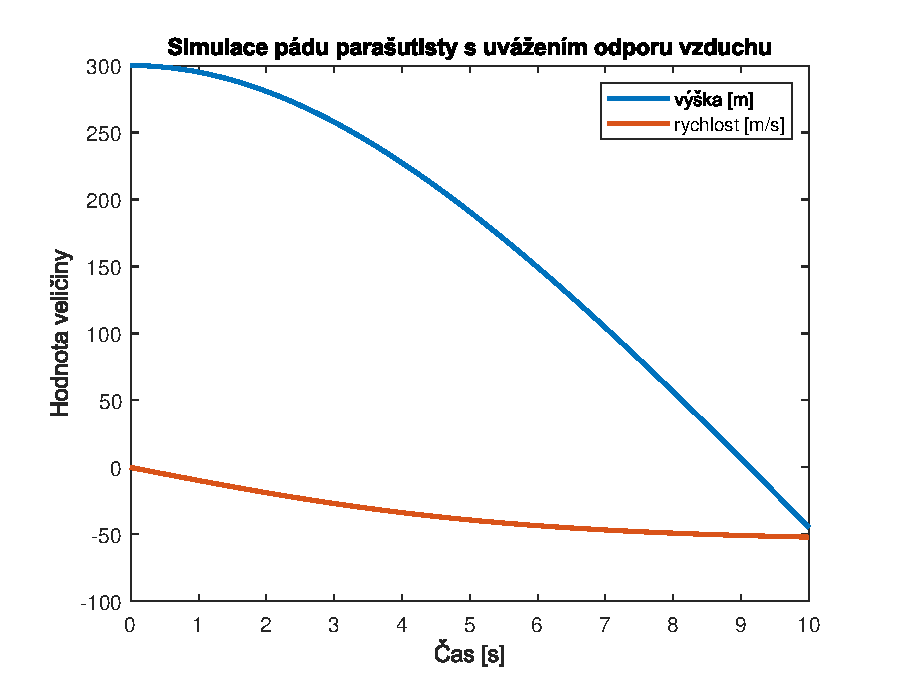
\includegraphics{parasutista.eps}
	\caption{Výstup simulace pádu parašutisty z úlohy 4 Matlabem}
	\label{fig:parasutista}
\end{figure}

\newpage
\section{Popis elektrického obvodu}
Napište soustavu algebro-diferenciálních rovnic pro zadané elektronické schéma uvedené v zadání.

\textbf{Řešení:}
V obvodu se nalézá sedm prvků, pro plné popsání bude potřeba 14 rovnic. Pasivní prvky jsou pojmenovány
$\text{R}_{1,2}$, $\text{C}_{1,2}$, $\text{L}$, zdroje proudu a napětí označím po řadě velkými písmeny I a U. 
Dále zápisy $i_x$ a $u_x$ představují po řadě proud a napětí na prvku $x$. Na obrázku \ref{fig:soustava_rovnic} jsou sepsané rovnice
a překreslené schéma s naznačenými orientacemi obvodových veličin. 

\begin{figure}[htb]
	\centering
	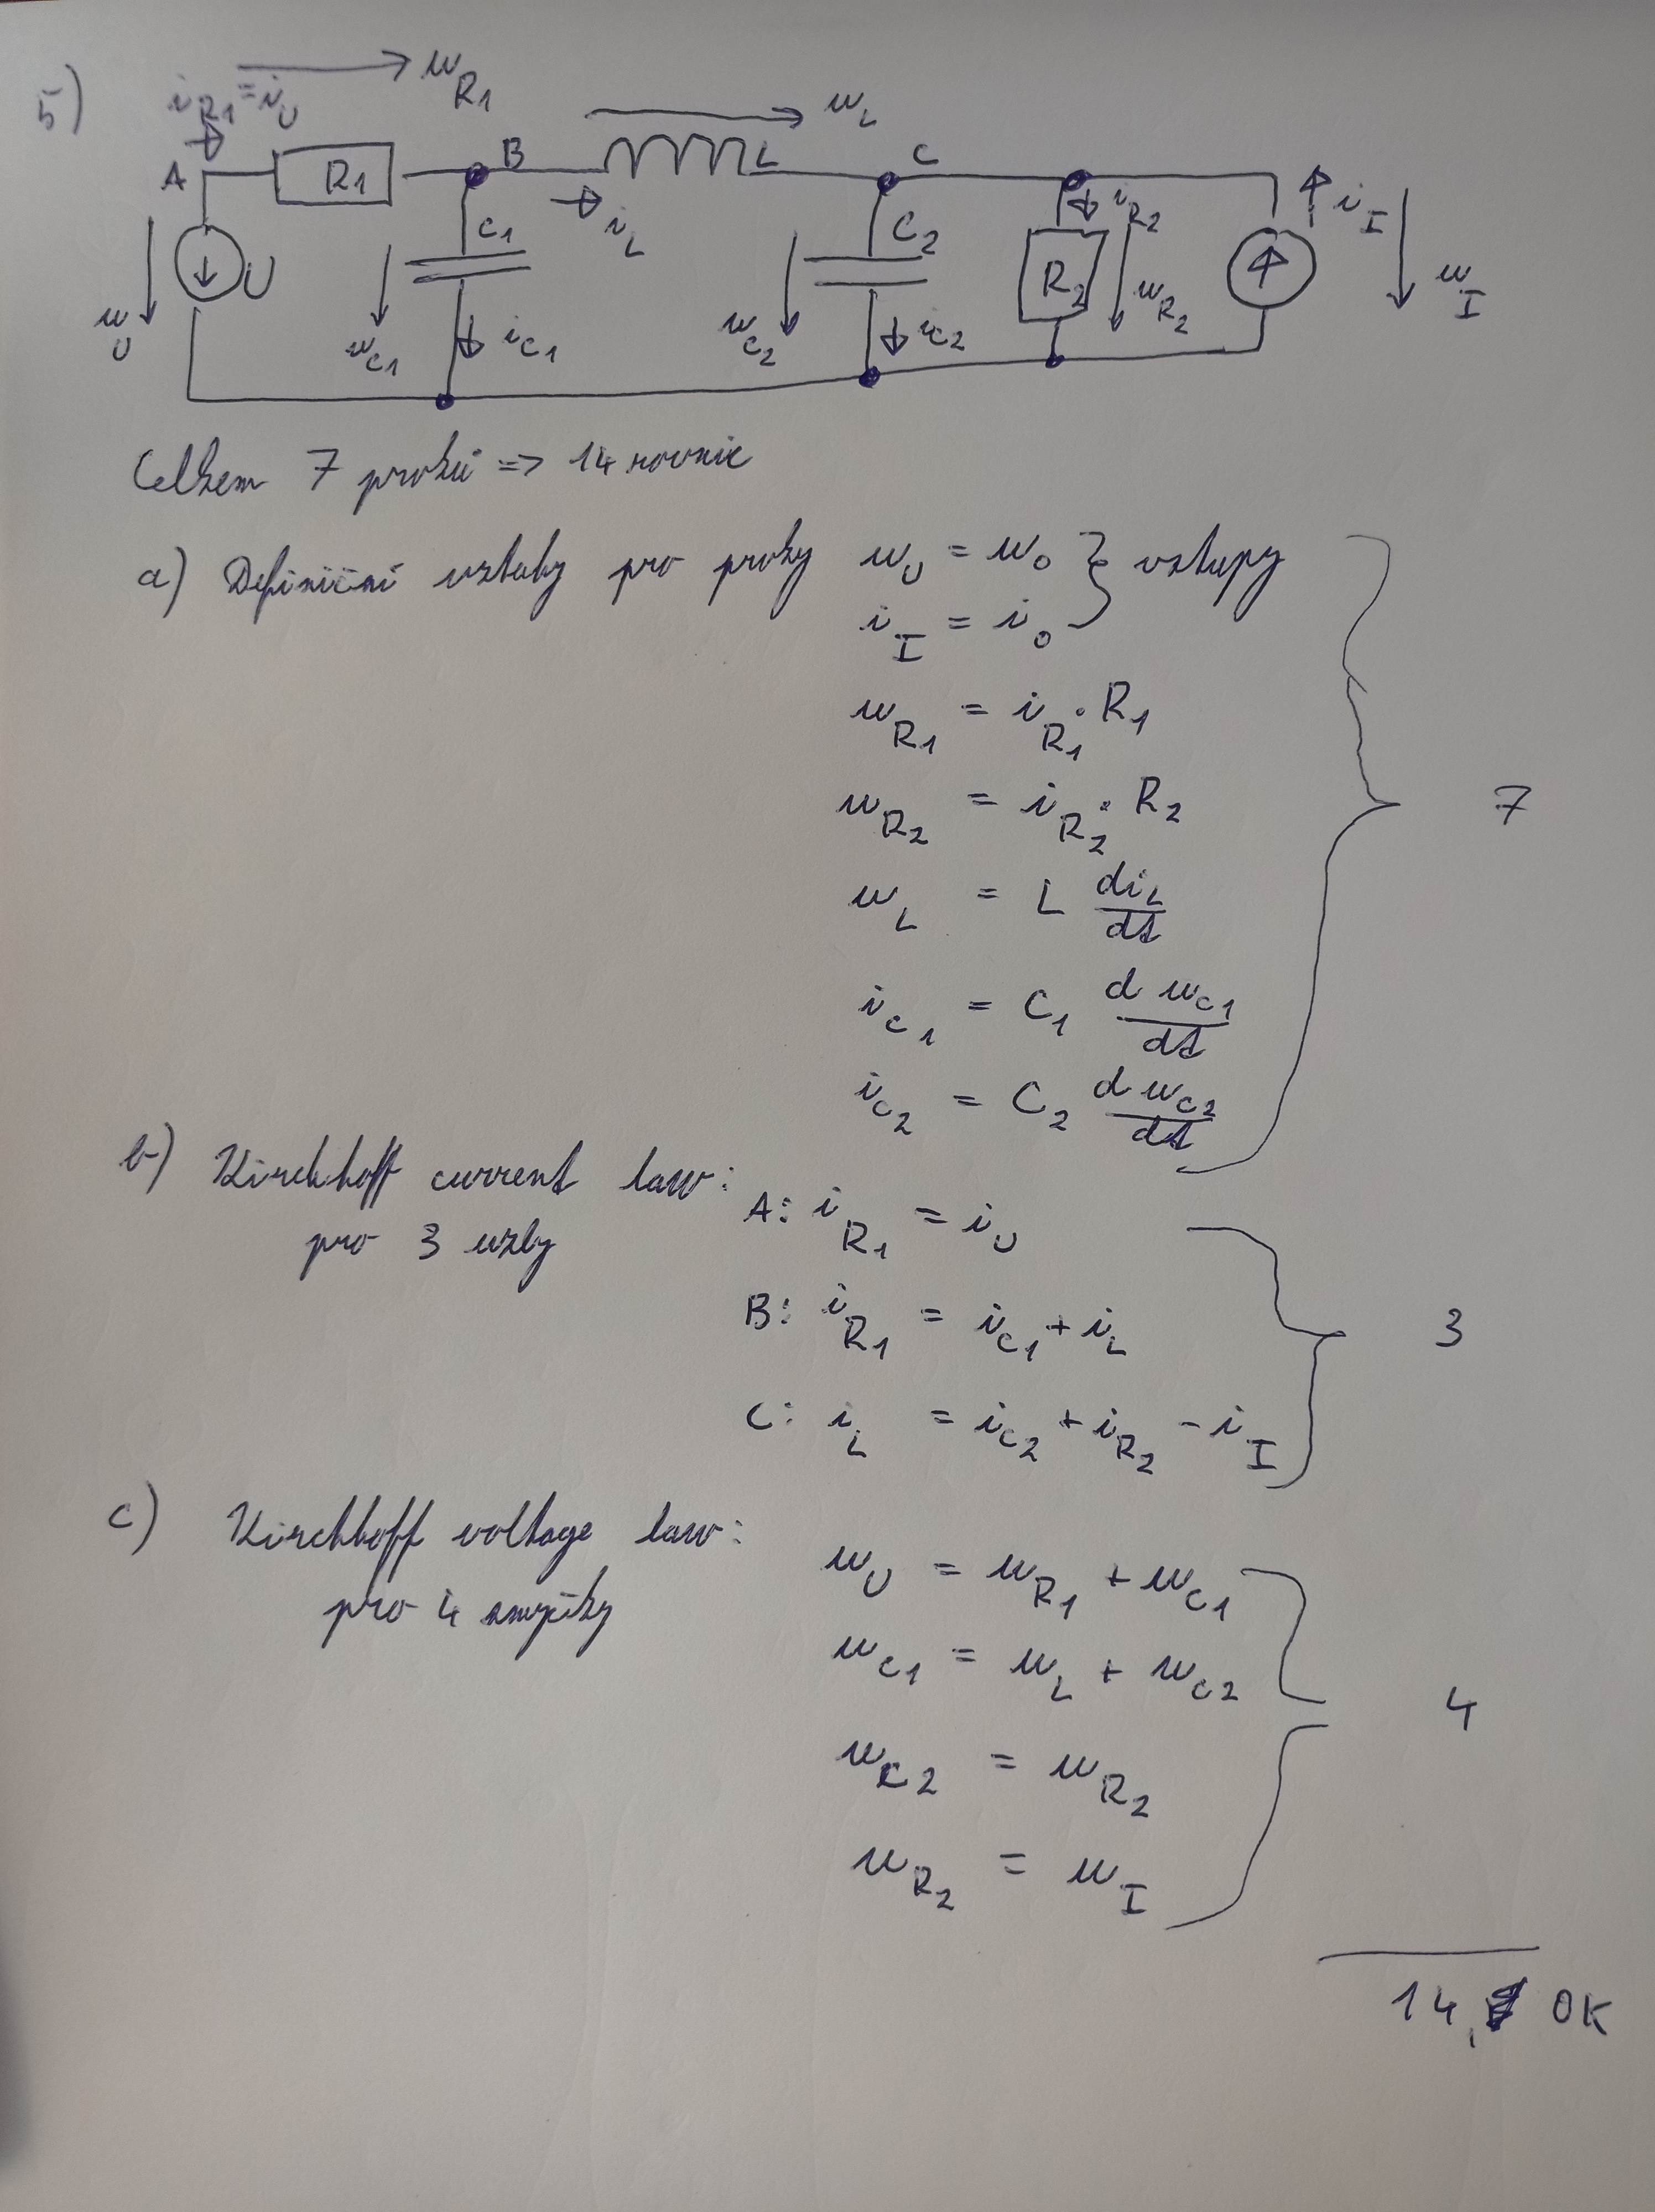
\includegraphics[width=.70\linewidth]{obvod_soustava_rovnic.jpg}
	\caption{Popis obvodu soustavou DAE}
	\label{fig:soustava_rovnic}
\end{figure}

\section{Simulace obvodu}
Simulujte odezvu na jednotkový skok v napětí $u_0$ pro obvod na schématu v zadání.
Parametry obvodu jsou: $L = 1.5 \text{ mH}$, $C =1 \text{ uF}$, $R = 100~\Omega$.
Jako výstupy zvolte proud protékající cívkou $L$ a napětí na kondenzátoru $C$.
V řešení uveďte graf s časovými průběhy výstupů včetně legendy a správných popisků os.

\textbf{Řešení:}
Pro simulaci obvodu je nezbytné pro něj vytvořit deskriptorový popis. Na obrázku \ref{fig:obvod_soustava_pro_simulaci} je
obkresleno schéma s naznačenou orientací veličin a rovnice ve formátu soustavy i ve zjednodušeném zápisu do matic $\mathbf{E}$, $\mathbf{A}$ a $\mathbf{B}$.

\begin{figure}[H]
	\centering
	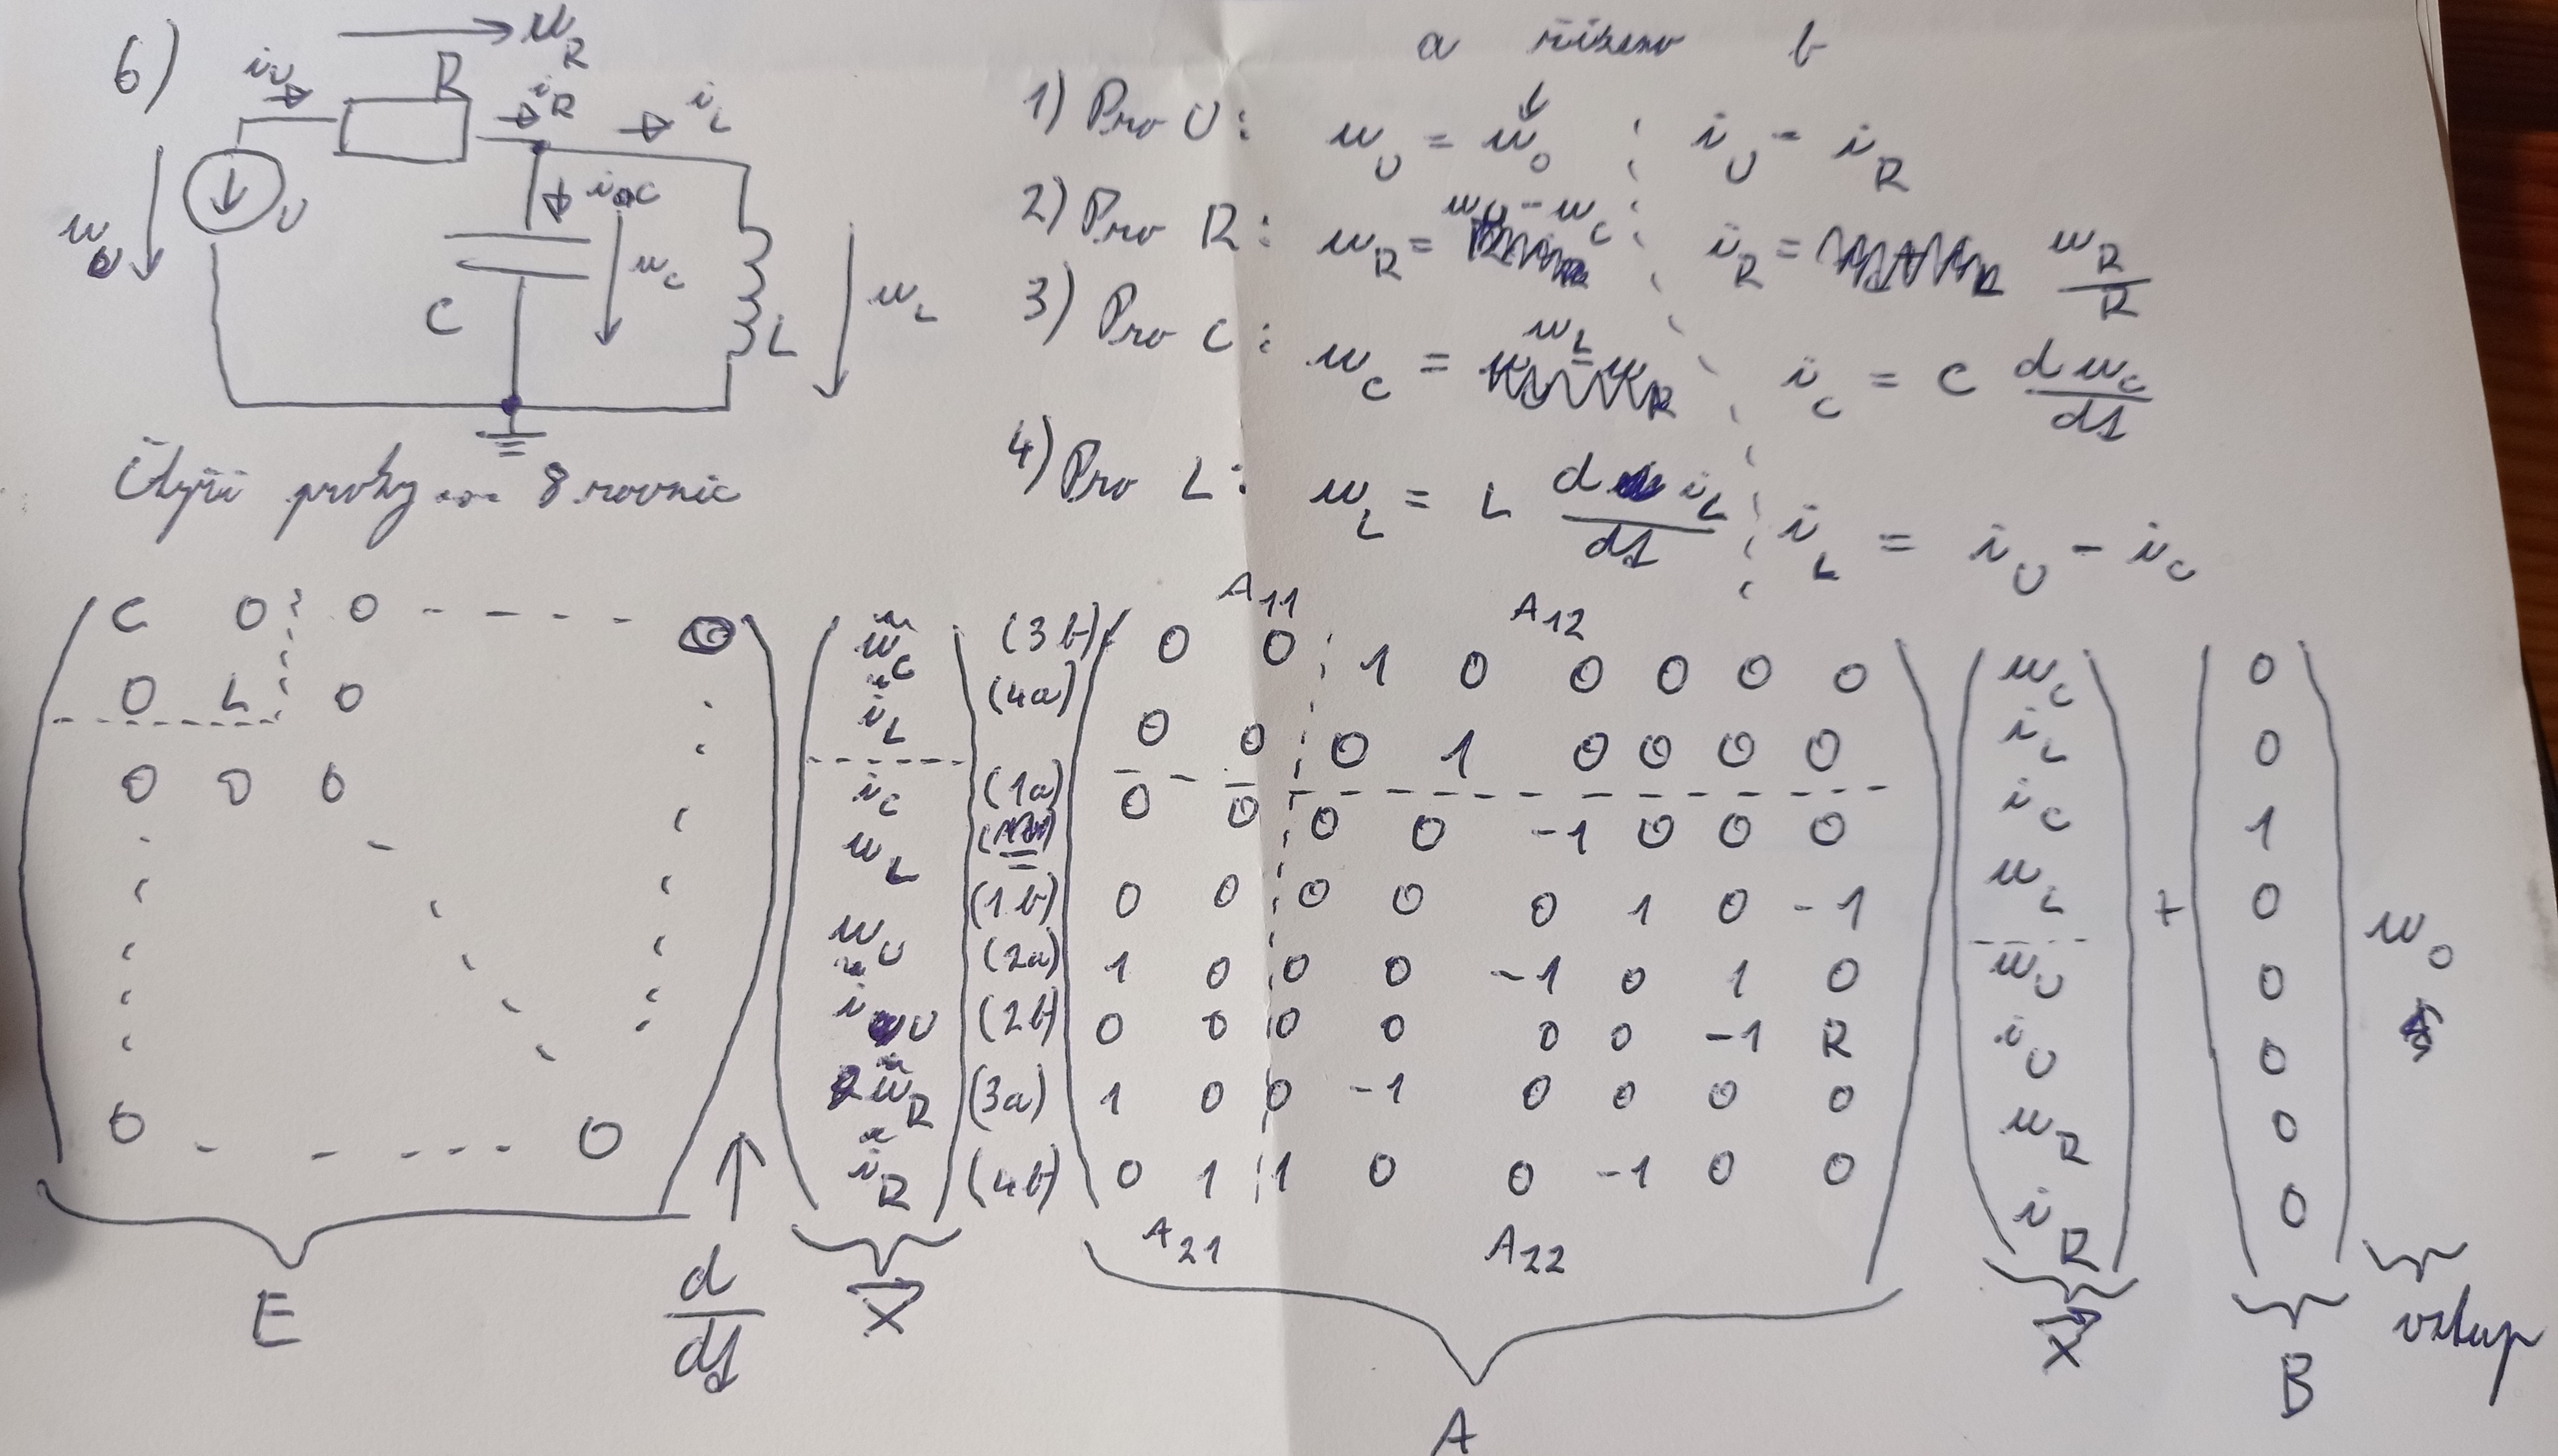
\includegraphics[width=.75\linewidth]{obvod_rovnice_pro_simulaci.jpg}
	\caption{DAE model obvodu pro simulaci}
	\label{fig:obvod_soustava_pro_simulaci}
\end{figure}

Na obrázku \ref{fig:obvod} je vykreslen výstup simulace. Správnost je složité ověřit detailně,
nicméně zhruba odpovídá očekávání. V čase $t < 0$ je obvod v klidu, netečou žádné proudy
a kondenzátor je vybit. Po odeznění přechodového děje ($t \to \infty$) bude induktor zkratován a poteče přes naj
proud omezený podle Ohmova zákona $i_{L_{\infty}} = \frac{u_0}{R} = 10 \text{ mA}$. Kapacitor
bude v ustáleném stavu otevřený obvod, jeho svorky budou zkratovány induktorem a proto bude $u_{C_\infty} = 0 \text{ V}$.
V průběhu ustalování se dá očekávat, že $C$ a $L$ si budou přelévat energii a obvod bude tlumeně oscilovat.

\begin{figure}[H]
	\centering
	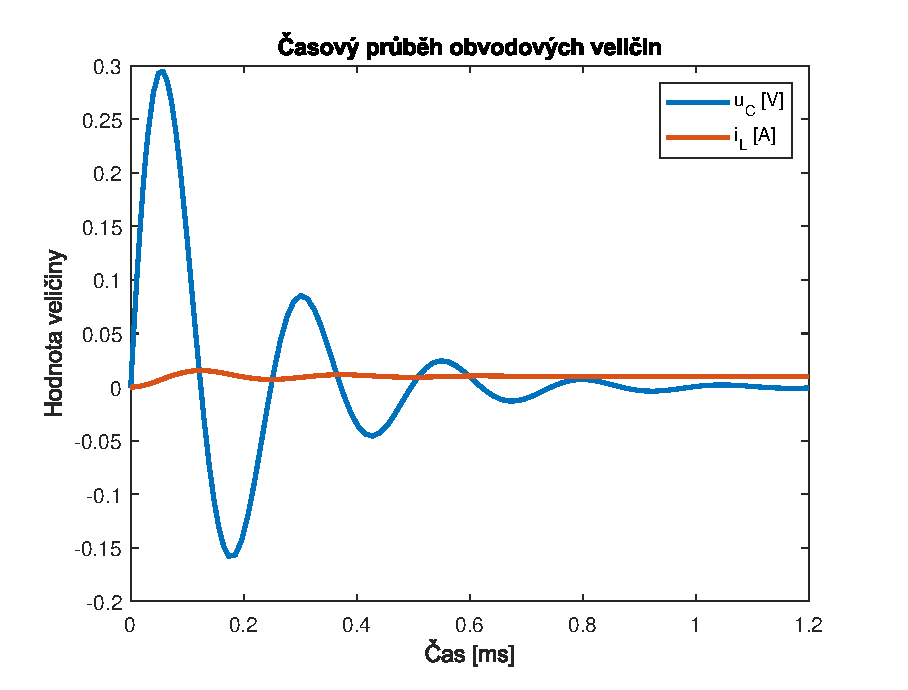
\includegraphics{obvod_prubehy.eps}
	\caption{Výstup simulace průběhu obvodových veličin pro úlohu 6 Matlabem}
	\label{fig:obvod}
\end{figure}
\newpage
\section{Převeďte model obvodu na stavové rovnice}
Převeďte model obvodu z příkladu č. 6 na stavové rovnice. Zdůvodněte, pokud to nelze

\textbf{Řešení:}
V úloze 6 byl nalezen model $\mathbf{E} \dot{\vec{x}} = \mathbf{A} \vec{x} + \mathbf{B} u_0$ s pseudostavem 
$\vec{x} = (\underbrace{u_C, i_L}_{\vec{x_1}^T}, \underbrace{i_C, u_L, u_U, i_U, u_R, i_R}_{\vec{x_2}^T})^T$ a maticemi
\begin{equation}
	\mathbf{E} = \left(\begin{array}{cc|cccccc}
		10^{-6} &        0          &  0      &   0      &   0      &   0      &   0       &  0 \\
		0       &1.5 \cdot 10^{-3}  &       0 &        0 &        0 &        0 &        0  &       0 \\
		\hline
		0       &               0   &      0  &       0  &       0  &       0  &       0   &      0 \\
		0       &               0   &      0  &       0  &       0  &       0  &       0   &      0 \\
		0       &               0   &      0  &       0  &       0  &       0  &       0   &      0 \\
		0       &               0   &      0  &       0  &       0  &       0  &       0   &      0 \\
		0       &               0   &      0  &       0  &       0  &       0  &       0   &      0 \\
		0       &               0   &      0  &       0  &       0  &       0  &       0   &      0 
	\end{array}\right), \mathbf{A} = \left( \begin{array}{cc|cccccc}
		
		0     & 0  &   1&     0  &   0 &    0 &    0 &    0 \\
		0     & 0  &   0&     1  &   0 &    0 &    0 &    0 \\
		\hline
		0     & 0  &   0&     0  &  -1 &    0 &    0 &    0 \\
		0     & 0  &   0&     0  &   0 &    1 &    0 &   -1 \\
		1     & 0  &   0&     0  &  -1 &    0 &    1 &    0 \\
		0     & 0  &   0&     0  &   0 &    0 &   -1 &  100 \\
		1     & 0  &   0&    -1  &   0 &    0 &    0 &    0 \\
		0     & 1  &   1&     0  &   0 &   -1 &    0 &    0
	\end{array}\right),\mathbf{B} = \left(\begin{array} {c}
		0 \\
		0 \\
		\hline
		1 \\
		0 \\
		0 \\
		0 \\
		0 \\
		0
	\end{array}\right).	
\end{equation}
Je naznačeno rozdělení vektoru $\vec{x}$ na dvě části $\vec{x}_{1,2}$ na diferenciální proměnné a ostatní proměnné.
Dále matice $\mathbf{A}$, $\mathbf{E}$, $\mathbf{B}$ jsou čarami rozděleny na podmatice, aby byly vizuálně oddělany části soustavy
operující s deferenciálními a "normálními" proměnnými. Na dílčí podmatice matice $\mathbf{H}$ se budu odkazovat
pomocí notace $\mathbf{H_{i,j}}$ (tučně jsou vyneseny indexy řádku $i$ a sloupce $j$). Například $\mathbf{A_{1,2}}$ je
matice $2 \times 6$ s hodnotami $\begin{bmatrix}
	1 & 0 & 0 & 0 & 0 &0 \\
	0 & 1 & 0 & 0 & 0 &0
\end{bmatrix}$.

S touto novou notací lze maticově zapsanou rovnici $\mathbf{E} \dot{\vec{x}} = \mathbf{A} \vec{x} + \mathbf{B} u_0$ přepsat po menších blocích
\begin{equation}
	\begin{split}
		\mathbf{E_{1,1}} \dot{\vec{x_1}} + \mathbf{E_{1,2}} \dot{\vec{x_2}} &= \mathbf{A_{1,1}} \vec{x_1} + \mathbf{A_{1,2}} \vec{x_2} + \mathbf{B_{1,1}} u_0, \\
		\mathbf{E_{2,1}} \dot{\vec{x_1}} + \mathbf{E_{2,2}} \dot{\vec{x_2}} &= \mathbf{A_{2,1}} \vec{x_1} + \mathbf{A_{2,2}} \vec{x_2} + \mathbf{B_{2,1}} u_0.
	\end{split}
\end{equation}
S vědomím, že v matici $\mathbf{E}$ je nenulová jen podmatice $\mathbf{E_{1,1}}$, lze odstranit nulové bloky a přeuspořádat členy na
\begin{equation}
	\begin{split}
		\mathbf{E_{1,1}} \dot{\vec{x_1}}  &= \mathbf{A_{1,1}} \vec{x_1} + \mathbf{A_{1,2}} \vec{x_2} + \mathbf{B_{1,1}} u_0, \\
		\mathbf{A_{2,2}} \vec{x_2} &= -\mathbf{A_{2,1}} \vec{x_1} - \mathbf{B_{2,1}} u_0.
		\label{eq:skoro_stavova}
	\end{split}
\end{equation}
Ze druhé rovnice lze za předpokladu invertovatelnosti $\mathbf{A_{2,2}}$ vyjádřit nediferenciální proměnné
\begin{equation}
	\vec{x_2} = -\mathbf{A_{2,2}}^{-1} (\mathbf{A_{2,1}} \vec{x_1} + \mathbf{B_{2,1}} u_0).
\end{equation}
Dosazením do \eqref{eq:skoro_stavova} získáme
\begin{equation}
	\mathbf{E_{1,1}} \dot{\vec{x_1}}  = \mathbf{A_{1,1}} \vec{x_1} - \mathbf{A_{1,2}} \mathbf{A_{2,2}}^{-1} (\mathbf{A_{2,1}} \vec{x_1} + \mathbf{B_{2,1}} u_0) + \mathbf{B_{1,1}} u_0.
	\label{eq:stavovy}
\end{equation}
Protože matice $\mathbf{E_{1,1}}$ je jistě regulární, bude možné ji invertovat. V rovnici \eqref{eq:statovy} dále seskupíme koeficienty
příslušné k $\vec{x_1}$ a $u0$ a osamostatníme $\dot{\vec{x_1}}$.
\begin{equation}
	\begin{split}
		\mathbf{E_{1,1}} \dot{\vec{x_1}}  &= \mathbf{A_{1,1}} \vec{x_1} - \mathbf{A_{1,2}} \mathbf{A_{2,2}}^{-1} \mathbf{A_{2,1}} \vec{x_1} - \mathbf{A_{1,2}} \mathbf{A_{2,2}}^{-1} \mathbf{B_{2,1}} u_0 + \mathbf{B_{1,1}} u_0 \\
		\mathbf{E_{1,1}} \dot{\vec{x_1}}  &= (\mathbf{A_{1,1}} - \mathbf{A_{1,2}} \mathbf{A_{2,2}}^{-1} \mathbf{A_{2,1}}) \vec{x_1} + (\mathbf{B_{1,1} - \mathbf{A_{1,2}} \mathbf{A_{2,2}}^{-1} \mathbf{B_{2,1}}}) u_0 \\
		\dot{\vec{x_1}}  &= \underbrace{\mathbf{E_{1,1}}^{-1}(\mathbf{A_{1,1}} - \mathbf{A_{1,2}} \mathbf{A_{2,2}}^{-1} \mathbf{A_{2,1}})}_{\mathbf{A_{\text{new}}}} \vec{x_1} + \underbrace{\mathbf{E_{1,1}}^{-1}(\mathbf{B_{1,1} - \mathbf{A_{1,2}} \mathbf{A_{2,2}}^{-1} \mathbf{B_{2,1}}})}_{\mathbf{B_{\text{new}}}} u_0 \\
	\end{split}
\end{equation}
Vyjádřením derivace stavů jako funkce $\dot{\vec{x_1}} = \dot{\vec{x_1}}(\vec{x_1}, u_0)$ byl získán stavový model. 
Vyčíslením matic $\mathbf{A_{\text{new}}}$ a $\mathbf{B_{\text{new}}}$ vychází stavový popis 
\begin{equation}
	\begin{bmatrix}
		\dot{u_C} \\
		\dot{i_L}
	\end{bmatrix} = \underbrace{\begin{bmatrix}
	-10^4 & -10^6 \\
	666.\bar{6} & 0	
\end{bmatrix}}_{\mathbf{A_{\text{new}}}} \begin{bmatrix}
	u_C \\ i_L
\end{bmatrix} + \underbrace{\begin{bmatrix}
	10^4 \\ 0
\end{bmatrix}}_{\mathbf{B_{\text{new}}}} u_0.
\end{equation}
\end{document}

